% Copyright 2019 Clara Eleonore Pavillet

% Author: Clara Eleonore Pavillet (original author), Leonard Quentin Marcq (modified for tsinghua), 赵宗义 (参与了修改), Li(modified for PKU)
% Description: This is an unofficial Peking University Beamer Template I made from scratch. Feel free to use it, modify it, share it.
% Repo Address: https://github.com/synthpop123/PKU-Beamer-Template
% Version: 1.1.1


\documentclass{beamer}
\usepackage{ctex}
\usepackage{fontspec}
% Load Packages
\usepackage[utf8]{inputenc}
\usepackage{xcolor}
\usepackage{tikz}
\usetikzlibrary{positioning,calc}
\usepackage{graphicx}
\usepackage{hyperref}
\usepackage{amsmath}
\usepackage{listings}
%\usepackage{fontawesome}

% Define Commands
\newcommand*{\ClipSep}{0.06cm} %To adjust footer logo
\newcommand{\E}{\mathrm{e}\,} %\def\I{e} % used to defined e for exp(x), see later what it should be
\newcommand{\ud}{\mathrm{d}}
\lstset{numbers=left, numberstyle=\tiny, stepnumber=1,firstnumber=1,breaklines=true,
    numbersep=5pt,language=Python,
    stringstyle=\ttfamily,
    basicstyle=\footnotesize, 
    showstringspaces=false
}

\usetheme{pku}

%%%<<<---
\newcommand{\system}{HashFlow}
\newcommand{\variable}{\mathrm}
\newcommand{\field}{\mathsf}
%%%--->>>

\title{\textbf{使用{\system}对计算机网络进行测量}}
\titlegraphic{
\includegraphics[width=2cm]{Theme/Logos/pku_emblem.png}}
\author{李康为}
\institute{北京大学计算机科学与技术系}
\date{} %\today

\begin{document}

{\setbeamertemplate{footline}{} 
\frame{\titlepage}}



\begin{frame}{{\system}的总体架构}
\textbf{控制平面}
\begin{enumerate}
\item 流记录项的分类和聚合
\item 流记录项的存储和分析
\end{enumerate}

\textbf{数据平面}
\begin{enumerate}
\item 哈希冲突解决策略
\item 大流检测机制
\item 不活跃流退出机制
\end{enumerate}
\end{frame}

\begin{frame}{数据平面}
\begin{enumerate}
\item 数据平面包含了两个哈希表, 分别是主表 (Main Table) 和辅表 (Ancillary Table).
\item 主表中每个哈希桶包含两个域: $\field{fieldID}$和$\field{count}$
\item 辅表中每个哈希桶也包含两个域: $\field{digest}$和$\field{count}$
\end{enumerate}
\begin{figure}
	\centering
	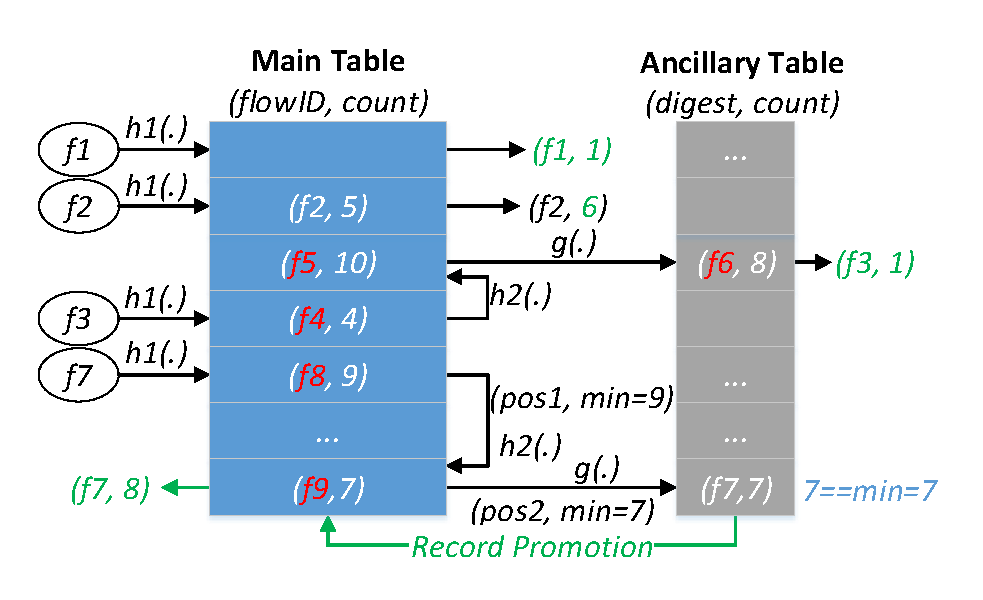
\includegraphics[width=0.6\linewidth]{figures/representation/datastructure}
\end{figure}

\end{frame}

  
\begin{frame}{}
\begin{center}
    \textbf{谢谢!}
\end{center}
\end{frame}


\end{document}

